% Draft chapter for kvis_final_research_report.tex (milestone M8).
% Insert with % Draft chapter for kvis_final_research_report.tex (milestone M8).
% Insert with % Draft chapter for kvis_final_research_report.tex (milestone M8).
% Insert with % Draft chapter for kvis_final_research_report.tex (milestone M8).
% Insert with \input{docs/report_drafts/results_title_alignment_20261106} immediately before
% \chapter{DISCUSSION}. It uses the report's own packages and column types (L, Y, booktabs, float).
% New references are in docs/report_drafts/references_additions_20261106.tex.
% Evidence tier: exploratory (Yahoo data, five starter stocks, validation years only). Numbers come
% from docs/long_term_reward_experiment_20261106.md, docs/walk_forward_reward_20261106.md and
% docs/source_ablation_20261106.md.

\chapter{LONG-TERM, MULTI-SOURCE EXTENSION}

This chapter reports experiments that align the implementation with the project title: a
\emph{long-term} objective, \emph{multi-source} inputs, and multi-year out-of-sample evaluation.
All results are exploratory. They use Yahoo Finance prices for the five starter stocks (ADVANC, AOT,
CPALL, KBANK, PTT) and the SET50 exchange-traded fund TDEX as the market series, because Yahoo now
returns only one row for the SET indices. Only validation years were read. The 2023--2024 test years
and the sealed post-2024 holdouts remain untouched for a single final evaluation after the protocol
is locked.

\section{Changes to the Environment and Objective}

The V2 environment charged turnover on the cash leg as well as on securities, so a 50\% purchase
from cash counted as 100\% turnover. It also reset portfolio weights to their targets after every
price move instead of letting them drift. Its reward was a one-day simple return minus a turnover
penalty of $0.05$ per unit of turnover, about fifty times the trading cost, and a penalty on the
\emph{level} of drawdown at every step. A new environment (\texttt{src/envs/long\_term\_env.py})
leaves the manifest-locked V2 files unchanged and adds opt-in options:

\begin{itemize}
  \item self-financing accounting with security-only turnover, multiplicative costs, and drifting weights;
  \item a log-wealth reward $\log(1+R_t)$, whose sum over an episode equals log terminal wealth;
  \item the plan reward $\alpha\log(1+R_t)+\beta D_t-\gamma\,\Delta\mathrm{DD}_t-\lambda\,\mathrm{TO}_t$, where $D_t$ is the differential Sharpe ratio of Moody and Saffell~\cite{moody2001drl} and only \emph{increases} in drawdown are penalized;
  \item a rebalancing interval, random two-year training episodes, and softmax portfolio weights with an explicit cash share.
\end{itemize}

With default options the new environment reproduced the V2 environment exactly. A randomized test
compares observations, rewards, and diagnostic values on random configurations. Trading costs were
set to 0.15\% commission plus 0.05\% slippage per side. That covers the published explicit cost of
about 0.176\% per side: a 0.157\% internet commission, SET, TSD, and SEC fees, and 7\% VAT.

\section{Reward and Rebalancing Designs (2020--2022)}

Six designs were trained with PPO for 100{,}000 timesteps and three seeds on 2012--2019. They were
evaluated on 2020--2022, which includes the COVID-19 crash, under self-financing accounting
(Table~\ref{tab:reward-designs}).

\begin{table}[H]
\centering
\small
\caption{Reward and rebalancing designs, validation 2020--2022 (mean $\pm$ s.d. over three seeds). Max DD is maximum drawdown, turnover is per session, and costs are commission plus slippage summed over the period as a share of portfolio value.}
\label{tab:reward-designs}
\begin{tabularx}{\textwidth}{@{}Yrrrr@{}}
\toprule
Design & Return & Max DD & Turnover & Costs \\
\midrule
V2 objective & $-48.8\% \pm 7.6$ & $-50.7\%$ & 0.519 & 75.3\% \\
Daily simple return, fixed accounting & $-41.9\% \pm 6.9$ & $-44.6\%$ & 0.386 & 56.0\% \\
Log return, weekly & $-2.8\% \pm 5.8$ & $-28.6\%$ & 0.110 & 16.0\% \\
Plan reward, weekly & $-8.8\% \pm 17.2$ & $-28.0\%$ & 0.081 & 11.7\% \\
Log return, monthly & $-5.2\% \pm 5.3$ & $-30.4\%$ & 0.031 & 4.5\% \\
Plan reward, weekly, LSTM model & $+1.9\% \pm 1.1$ & $-26.0\%$ & 0.011 & 1.6\% \\
\midrule
SET50 ETF buy-and-hold & $+9.0\%$ & $-32.6\%$ & -- & 0.2\% \\
Ridge forecast, top two, monthly & $+4.9\%$ & $-33.2\%$ & 0.050 & 7.3\% \\
Equal weight, monthly & $+2.7\%$ & $-31.6\%$ & 0.003 & 0.5\% \\
\bottomrule
\end{tabularx}
\end{table}

The V2 objective lost money mainly through overtrading: its policy turned over the portfolio about
377 times in three years. Correcting the accounting alone did not help, because a daily-decision agent
still churned. Long-horizon rewards with weekly or monthly decisions cut costs by 79--94\% and
reduced the loss from about 49\% to about 3\%. A shared per-asset LSTM encoder of each stock's
\emph{past} window (\texttt{asset\_lstm}) gave the only design that was positive on every seed.

\section{Seven-Year Walk-Forward Evaluation}

The two carried-forward designs were re-evaluated with seven expanding folds. Each fold trained on
2012 through December of year $Y-1$ and validated on year $Y$ ($Y=2016,\dots,2022$), with five seeds per
design. Two supervised forecast-then-allocate baselines were fitted on the same training dates: a ridge
regression and a bidirectional LSTM over each stock's past window. Each predicted 21-session returns
and bought its top two forecasts monthly. Table~\ref{tab:walk-forward} summarizes the folds.

\begin{table}[H]
\centering
\small
\caption{Walk-forward validation 2016--2022: mean over seven annual folds (DRL: five seeds per fold).}
\label{tab:walk-forward}
\begin{tabularx}{\textwidth}{@{}Yrrrr@{}}
\toprule
Strategy & Annual return & vs ETF & Years ahead & Max DD \\
\midrule
LSTM forecast, top two & 13.8\% & $+6.7\%$ & 5/7 & $-17.0\%$ \\
Ridge forecast, top two & 12.8\% & $+5.6\%$ & 5/7 & $-16.8\%$ \\
Equal weight, monthly & 10.1\% & $+3.0\%$ & 4/7 & $-13.9\%$ \\
DRL, plan reward + LSTM model & 7.7\% & $+0.5\%$ & 3/7 & $-11.1\%$ \\
SET50 ETF buy-and-hold & 7.1\% & -- & -- & $-11.3\%$ \\
DRL, log reward + MLP & 5.0\% & $-2.2\%$ & 2/7 & $-14.2\%$ \\
\bottomrule
\end{tabularx}
\end{table}

\begin{figure}[H]
\centering
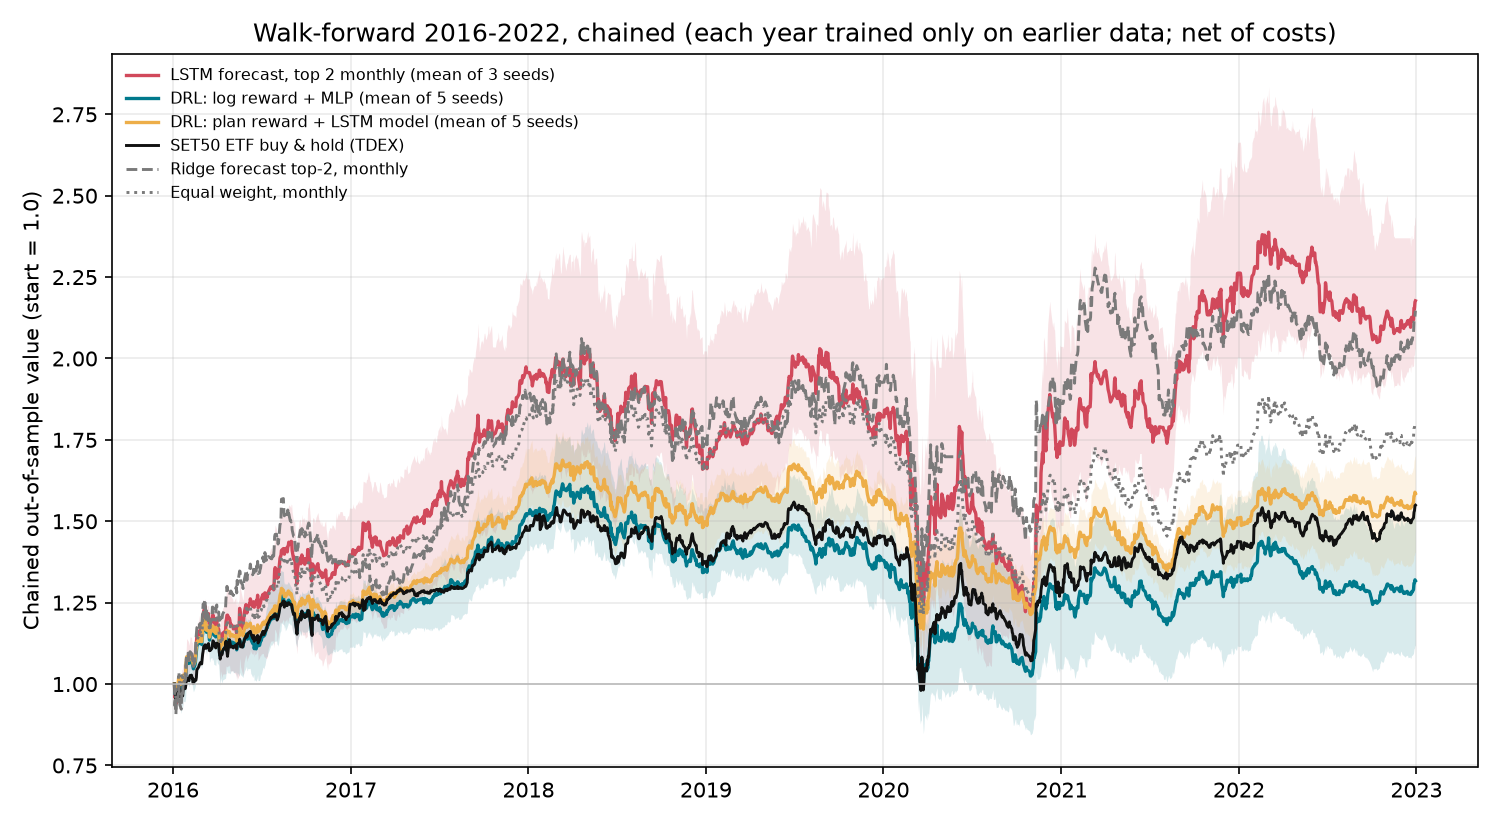
\includegraphics[width=\textwidth]{docs/figures/walk_forward_chained_equity_20261106.png}
\caption{Chained out-of-sample value over the seven validation years. Each year uses models trained only on earlier years. Bands show the range across seeds.}
\label{fig:walk-forward}
\end{figure}

Uncertainty was assessed on chained daily returns with a stationary block bootstrap~\cite{politis1994stationary},
the probabilistic Sharpe ratio~\cite{bailey2012sharpe}, and the deflated Sharpe ratio~\cite{bailey2014deflated},
counting the six designs screened earlier. The DRL LSTM agent had an annualized Sharpe ratio of 0.55
(95\% interval $-0.20$ to $1.32$) against 0.50 for the ETF. The paired difference was $+0.05$
(95\% interval $-0.29$ to $0.36$), and its deflated Sharpe ratio was 0.55, close to the value expected
from the best of six unskilled designs. The only difference whose interval excluded zero was that the
MLP agent was worse than equal weight (Sharpe difference $-0.24$, 95\% interval $-0.41$ to $-0.10$).

\section{Data-Source Ablation and Attribution}

With the reward, model, seeds, and folds fixed, the agent's inputs were varied (Table~\ref{tab:ablation}).

\begin{table}[H]
\centering
\small
\caption{Data-source ablation over the seven walk-forward years (three seeds per arm).}
\label{tab:ablation}
\begin{tabularx}{\textwidth}{@{}Yrrrr@{}}
\toprule
Inputs & Features & Annual return & vs ETF & Years ahead \\
\midrule
Technical only & 11 & 6.8\% & $-0.3\%$ & 3/7 \\
Technical + SET50 market context & 16 & 8.2\% & $+1.1\%$ & 4/7 \\
+ daily macro proxies & 24 & 7.1\% & $-0.1\%$ & 3/7 \\
\bottomrule
\end{tabularx}
\end{table}

\begin{figure}[H]
\centering
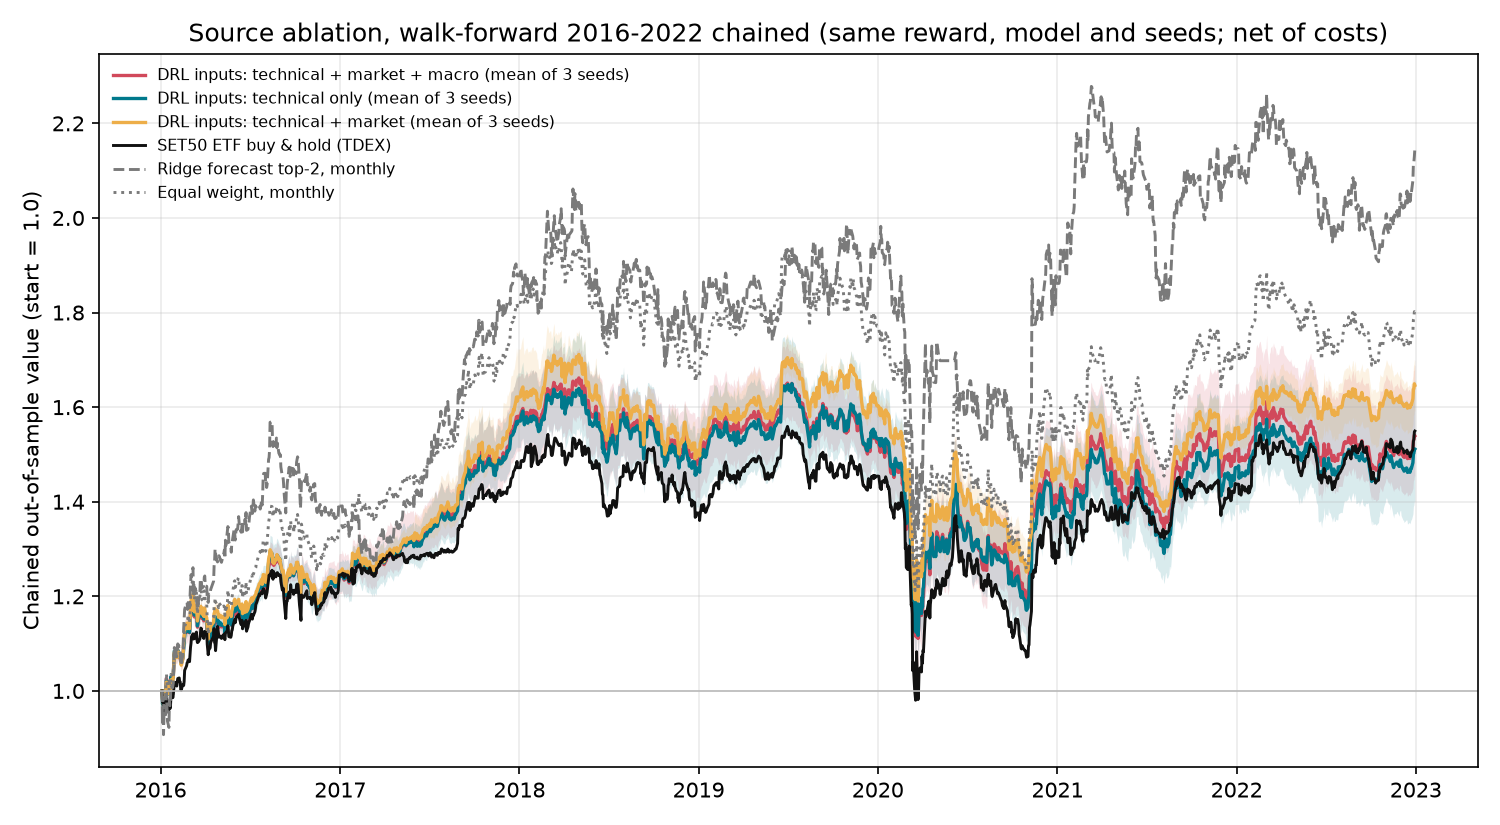
\includegraphics[width=\textwidth]{docs/figures/source_ablation_chained_equity_20261106.png}
\caption{Source ablation: chained out-of-sample value of the same DRL design with three input sets (three seeds each), compared with the ETF, equal weight, and the ridge forecast.}
\label{fig:ablation}
\end{figure}

Adding market context raised the Sharpe ratio by 0.10 relative to technical inputs only (95\% interval
$-0.002$ to $0.21$, one-sided $p=0.03$). That is borderline evidence, and it would not survive a
correction for the three comparisons. Daily macro proxies (USD/THB, Brent, gold, and the US 10-year
yield) added nothing.

Permutation attribution shuffled each source group in time and re-ran the trained agents. The macro
inputs moved the agent's weights by 2.9\%, the technical inputs by 5.5\%, and the market inputs by
1.9\%, but none changed annual return by more than 0.25 percentage points. In the main walk-forward
the LSTM agent's weights moved only 5.8\% (technical) and 2.5\% (market), so it behaved close to a
stable allocation. The MLP agent reacted strongly (27\% and 19\%) but lost more to trading costs (5.3\%
a year) than it gained from its inputs.

\section{Algorithm Comparison}

PPO was compared with A2C~\cite{mnih2016a3c} under the same reward, model, inputs, folds, and seeds
(Table~\ref{tab:algorithms}). PPO earned 0.9 percentage points more per year, beat the ETF in four of
seven years, and had the shallower drawdown. Most of its advantage came after the 2020 crash. The
Sharpe difference was not significant ($-0.11$ for A2C relative to PPO, 95\% interval $-0.26$ to
$0.04$). A2C trained about four times faster. The off-policy algorithms SAC~\cite{haarnoja2018sac},
TD3~\cite{fujimoto2018td3}, and DDPG~\cite{lillicrap2015ddpg} require about one hour per run and about
1~GB of replay memory with this model, so their comparison is prepared as an HPC array job rather
than run on the 8~GB development machine.

\begin{table}[H]
\centering
\small
\caption{On-policy algorithm comparison over the seven walk-forward years (three seeds each, same reward and model).}
\label{tab:algorithms}
\begin{tabularx}{\textwidth}{@{}Yrrrr@{}}
\toprule
Algorithm & Annual return & vs ETF & Years ahead & Max DD \\
\midrule
PPO & 8.2\% & $+1.1\%$ & 4/7 & $-11.1\%$ \\
A2C & 7.3\% & $+0.2\%$ & 3/7 & $-13.2\%$ \\
SET50 ETF buy-and-hold & 7.1\% & -- & -- & $-11.3\%$ \\
\bottomrule
\end{tabularx}
\end{table}

\section{Interpretation}

The long-term DRL design fixed the overtrading failure of the V2 objective. Over seven years it
roughly matched the SET50 market with the lowest drawdown of any strategy tested. However, it did not
outperform equal weighting of the same stocks or the supervised forecast-then-allocate baselines, and
no comparison among these strategies was statistically significant. The five starter stocks are
current large capitalization survivors chosen with hindsight, so even their equal-weight portfolio
outperformed the market index. Extending the evaluation to the point-in-time SET50/SET100 universe,
and adding fundamentals, news sentiment, investor flow, and official point-in-time macro data, are
required before any claim about Thai markets in general.
 immediately before
% \chapter{DISCUSSION}. It uses the report's own packages and column types (L, Y, booktabs, float).
% New references are in docs/report_drafts/references_additions_20261106.tex.
% Evidence tier: exploratory (Yahoo data, five starter stocks, validation years only). Numbers come
% from docs/long_term_reward_experiment_20261106.md, docs/walk_forward_reward_20261106.md and
% docs/source_ablation_20261106.md.

\chapter{LONG-TERM, MULTI-SOURCE EXTENSION}

This chapter reports experiments that align the implementation with the project title: a
\emph{long-term} objective, \emph{multi-source} inputs, and multi-year out-of-sample evaluation.
All results are exploratory. They use Yahoo Finance prices for the five starter stocks (ADVANC, AOT,
CPALL, KBANK, PTT) and the SET50 exchange-traded fund TDEX as the market series, because Yahoo now
returns only one row for the SET indices. Only validation years were read. The 2023--2024 test years
and the sealed post-2024 holdouts remain untouched for a single final evaluation after the protocol
is locked.

\section{Changes to the Environment and Objective}

The V2 environment charged turnover on the cash leg as well as on securities, so a 50\% purchase
from cash counted as 100\% turnover. It also reset portfolio weights to their targets after every
price move instead of letting them drift. Its reward was a one-day simple return minus a turnover
penalty of $0.05$ per unit of turnover, about fifty times the trading cost, and a penalty on the
\emph{level} of drawdown at every step. A new environment (\texttt{src/envs/long\_term\_env.py})
leaves the manifest-locked V2 files unchanged and adds opt-in options:

\begin{itemize}
  \item self-financing accounting with security-only turnover, multiplicative costs, and drifting weights;
  \item a log-wealth reward $\log(1+R_t)$, whose sum over an episode equals log terminal wealth;
  \item the plan reward $\alpha\log(1+R_t)+\beta D_t-\gamma\,\Delta\mathrm{DD}_t-\lambda\,\mathrm{TO}_t$, where $D_t$ is the differential Sharpe ratio of Moody and Saffell~\cite{moody2001drl} and only \emph{increases} in drawdown are penalized;
  \item a rebalancing interval, random two-year training episodes, and softmax portfolio weights with an explicit cash share.
\end{itemize}

With default options the new environment reproduced the V2 environment exactly. A randomized test
compares observations, rewards, and diagnostic values on random configurations. Trading costs were
set to 0.15\% commission plus 0.05\% slippage per side. That covers the published explicit cost of
about 0.176\% per side: a 0.157\% internet commission, SET, TSD, and SEC fees, and 7\% VAT.

\section{Reward and Rebalancing Designs (2020--2022)}

Six designs were trained with PPO for 100{,}000 timesteps and three seeds on 2012--2019. They were
evaluated on 2020--2022, which includes the COVID-19 crash, under self-financing accounting
(Table~\ref{tab:reward-designs}).

\begin{table}[H]
\centering
\small
\caption{Reward and rebalancing designs, validation 2020--2022 (mean $\pm$ s.d. over three seeds). Max DD is maximum drawdown, turnover is per session, and costs are commission plus slippage summed over the period as a share of portfolio value.}
\label{tab:reward-designs}
\begin{tabularx}{\textwidth}{@{}Yrrrr@{}}
\toprule
Design & Return & Max DD & Turnover & Costs \\
\midrule
V2 objective & $-48.8\% \pm 7.6$ & $-50.7\%$ & 0.519 & 75.3\% \\
Daily simple return, fixed accounting & $-41.9\% \pm 6.9$ & $-44.6\%$ & 0.386 & 56.0\% \\
Log return, weekly & $-2.8\% \pm 5.8$ & $-28.6\%$ & 0.110 & 16.0\% \\
Plan reward, weekly & $-8.8\% \pm 17.2$ & $-28.0\%$ & 0.081 & 11.7\% \\
Log return, monthly & $-5.2\% \pm 5.3$ & $-30.4\%$ & 0.031 & 4.5\% \\
Plan reward, weekly, LSTM model & $+1.9\% \pm 1.1$ & $-26.0\%$ & 0.011 & 1.6\% \\
\midrule
SET50 ETF buy-and-hold & $+9.0\%$ & $-32.6\%$ & -- & 0.2\% \\
Ridge forecast, top two, monthly & $+4.9\%$ & $-33.2\%$ & 0.050 & 7.3\% \\
Equal weight, monthly & $+2.7\%$ & $-31.6\%$ & 0.003 & 0.5\% \\
\bottomrule
\end{tabularx}
\end{table}

The V2 objective lost money mainly through overtrading: its policy turned over the portfolio about
377 times in three years. Correcting the accounting alone did not help, because a daily-decision agent
still churned. Long-horizon rewards with weekly or monthly decisions cut costs by 79--94\% and
reduced the loss from about 49\% to about 3\%. A shared per-asset LSTM encoder of each stock's
\emph{past} window (\texttt{asset\_lstm}) gave the only design that was positive on every seed.

\section{Seven-Year Walk-Forward Evaluation}

The two carried-forward designs were re-evaluated with seven expanding folds. Each fold trained on
2012 through December of year $Y-1$ and validated on year $Y$ ($Y=2016,\dots,2022$), with five seeds per
design. Two supervised forecast-then-allocate baselines were fitted on the same training dates: a ridge
regression and a bidirectional LSTM over each stock's past window. Each predicted 21-session returns
and bought its top two forecasts monthly. Table~\ref{tab:walk-forward} summarizes the folds.

\begin{table}[H]
\centering
\small
\caption{Walk-forward validation 2016--2022: mean over seven annual folds (DRL: five seeds per fold).}
\label{tab:walk-forward}
\begin{tabularx}{\textwidth}{@{}Yrrrr@{}}
\toprule
Strategy & Annual return & vs ETF & Years ahead & Max DD \\
\midrule
LSTM forecast, top two & 13.8\% & $+6.7\%$ & 5/7 & $-17.0\%$ \\
Ridge forecast, top two & 12.8\% & $+5.6\%$ & 5/7 & $-16.8\%$ \\
Equal weight, monthly & 10.1\% & $+3.0\%$ & 4/7 & $-13.9\%$ \\
DRL, plan reward + LSTM model & 7.7\% & $+0.5\%$ & 3/7 & $-11.1\%$ \\
SET50 ETF buy-and-hold & 7.1\% & -- & -- & $-11.3\%$ \\
DRL, log reward + MLP & 5.0\% & $-2.2\%$ & 2/7 & $-14.2\%$ \\
\bottomrule
\end{tabularx}
\end{table}

\begin{figure}[H]
\centering
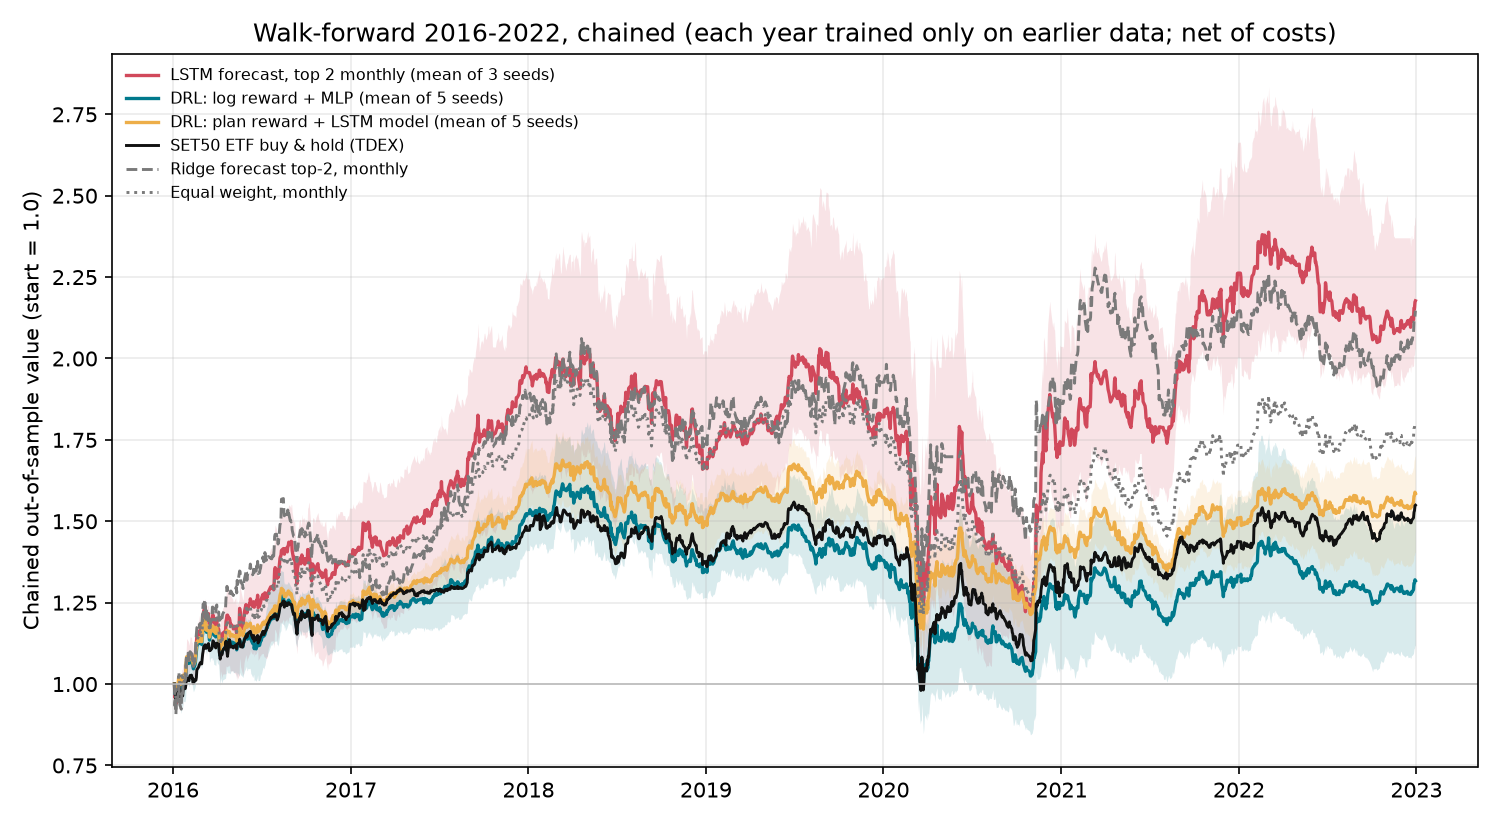
\includegraphics[width=\textwidth]{docs/figures/walk_forward_chained_equity_20261106.png}
\caption{Chained out-of-sample value over the seven validation years. Each year uses models trained only on earlier years. Bands show the range across seeds.}
\label{fig:walk-forward}
\end{figure}

Uncertainty was assessed on chained daily returns with a stationary block bootstrap~\cite{politis1994stationary},
the probabilistic Sharpe ratio~\cite{bailey2012sharpe}, and the deflated Sharpe ratio~\cite{bailey2014deflated},
counting the six designs screened earlier. The DRL LSTM agent had an annualized Sharpe ratio of 0.55
(95\% interval $-0.20$ to $1.32$) against 0.50 for the ETF. The paired difference was $+0.05$
(95\% interval $-0.29$ to $0.36$), and its deflated Sharpe ratio was 0.55, close to the value expected
from the best of six unskilled designs. The only difference whose interval excluded zero was that the
MLP agent was worse than equal weight (Sharpe difference $-0.24$, 95\% interval $-0.41$ to $-0.10$).

\section{Data-Source Ablation and Attribution}

With the reward, model, seeds, and folds fixed, the agent's inputs were varied (Table~\ref{tab:ablation}).

\begin{table}[H]
\centering
\small
\caption{Data-source ablation over the seven walk-forward years (three seeds per arm).}
\label{tab:ablation}
\begin{tabularx}{\textwidth}{@{}Yrrrr@{}}
\toprule
Inputs & Features & Annual return & vs ETF & Years ahead \\
\midrule
Technical only & 11 & 6.8\% & $-0.3\%$ & 3/7 \\
Technical + SET50 market context & 16 & 8.2\% & $+1.1\%$ & 4/7 \\
+ daily macro proxies & 24 & 7.1\% & $-0.1\%$ & 3/7 \\
\bottomrule
\end{tabularx}
\end{table}

\begin{figure}[H]
\centering
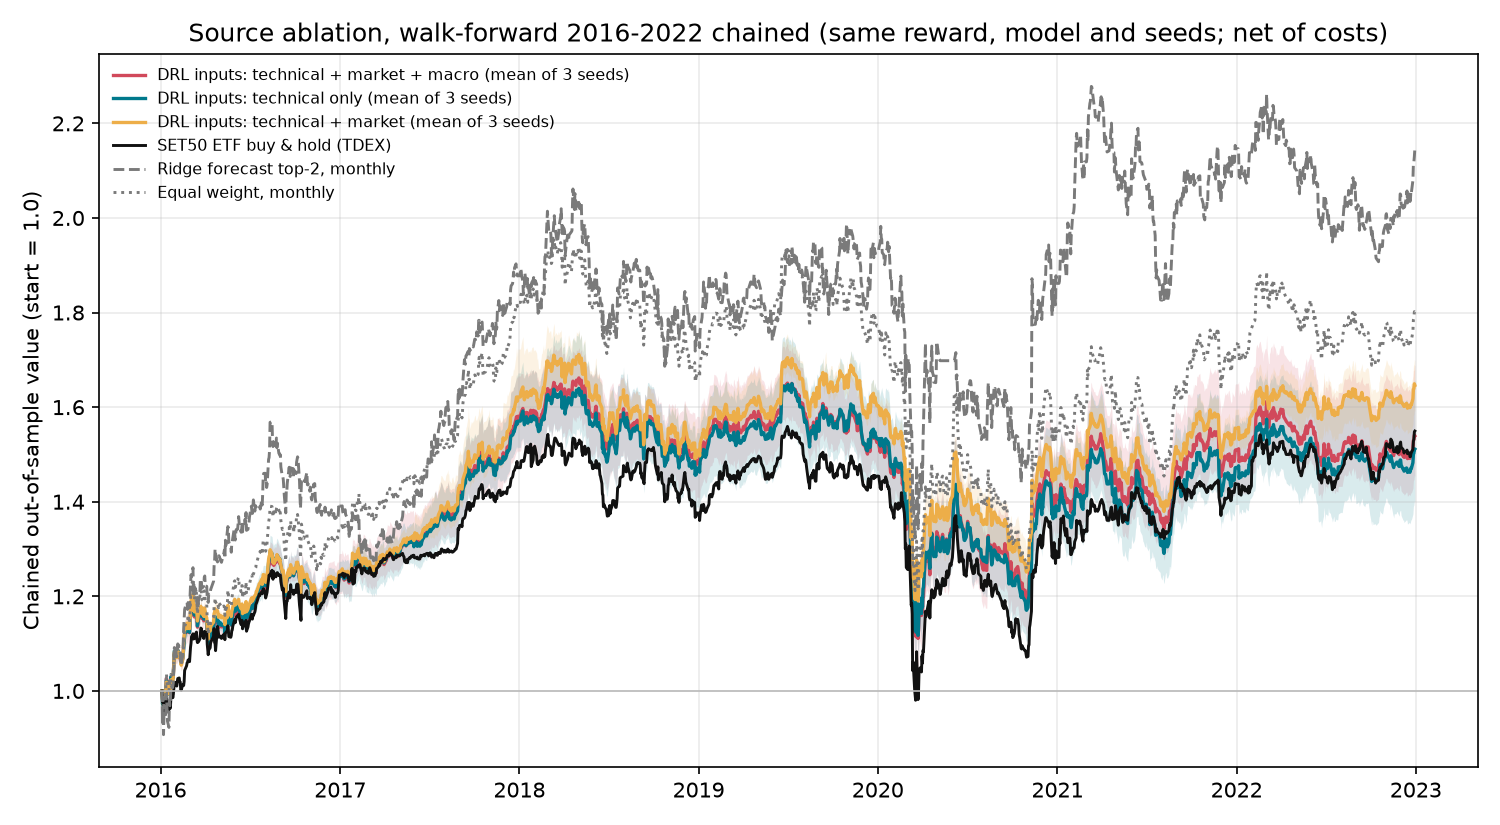
\includegraphics[width=\textwidth]{docs/figures/source_ablation_chained_equity_20261106.png}
\caption{Source ablation: chained out-of-sample value of the same DRL design with three input sets (three seeds each), compared with the ETF, equal weight, and the ridge forecast.}
\label{fig:ablation}
\end{figure}

Adding market context raised the Sharpe ratio by 0.10 relative to technical inputs only (95\% interval
$-0.002$ to $0.21$, one-sided $p=0.03$). That is borderline evidence, and it would not survive a
correction for the three comparisons. Daily macro proxies (USD/THB, Brent, gold, and the US 10-year
yield) added nothing.

Permutation attribution shuffled each source group in time and re-ran the trained agents. The macro
inputs moved the agent's weights by 2.9\%, the technical inputs by 5.5\%, and the market inputs by
1.9\%, but none changed annual return by more than 0.25 percentage points. In the main walk-forward
the LSTM agent's weights moved only 5.8\% (technical) and 2.5\% (market), so it behaved close to a
stable allocation. The MLP agent reacted strongly (27\% and 19\%) but lost more to trading costs (5.3\%
a year) than it gained from its inputs.

\section{Algorithm Comparison}

PPO was compared with A2C~\cite{mnih2016a3c} under the same reward, model, inputs, folds, and seeds
(Table~\ref{tab:algorithms}). PPO earned 0.9 percentage points more per year, beat the ETF in four of
seven years, and had the shallower drawdown. Most of its advantage came after the 2020 crash. The
Sharpe difference was not significant ($-0.11$ for A2C relative to PPO, 95\% interval $-0.26$ to
$0.04$). A2C trained about four times faster. The off-policy algorithms SAC~\cite{haarnoja2018sac},
TD3~\cite{fujimoto2018td3}, and DDPG~\cite{lillicrap2015ddpg} require about one hour per run and about
1~GB of replay memory with this model, so their comparison is prepared as an HPC array job rather
than run on the 8~GB development machine.

\begin{table}[H]
\centering
\small
\caption{On-policy algorithm comparison over the seven walk-forward years (three seeds each, same reward and model).}
\label{tab:algorithms}
\begin{tabularx}{\textwidth}{@{}Yrrrr@{}}
\toprule
Algorithm & Annual return & vs ETF & Years ahead & Max DD \\
\midrule
PPO & 8.2\% & $+1.1\%$ & 4/7 & $-11.1\%$ \\
A2C & 7.3\% & $+0.2\%$ & 3/7 & $-13.2\%$ \\
SET50 ETF buy-and-hold & 7.1\% & -- & -- & $-11.3\%$ \\
\bottomrule
\end{tabularx}
\end{table}

\section{Interpretation}

The long-term DRL design fixed the overtrading failure of the V2 objective. Over seven years it
roughly matched the SET50 market with the lowest drawdown of any strategy tested. However, it did not
outperform equal weighting of the same stocks or the supervised forecast-then-allocate baselines, and
no comparison among these strategies was statistically significant. The five starter stocks are
current large capitalization survivors chosen with hindsight, so even their equal-weight portfolio
outperformed the market index. Extending the evaluation to the point-in-time SET50/SET100 universe,
and adding fundamentals, news sentiment, investor flow, and official point-in-time macro data, are
required before any claim about Thai markets in general.
 immediately before
% \chapter{DISCUSSION}. It uses the report's own packages and column types (L, Y, booktabs, float).
% New references are in docs/report_drafts/references_additions_20261106.tex.
% Evidence tier: exploratory (Yahoo data, five starter stocks, validation years only). Numbers come
% from docs/long_term_reward_experiment_20261106.md, docs/walk_forward_reward_20261106.md and
% docs/source_ablation_20261106.md.

\chapter{LONG-TERM, MULTI-SOURCE EXTENSION}

This chapter reports experiments that align the implementation with the project title: a
\emph{long-term} objective, \emph{multi-source} inputs, and multi-year out-of-sample evaluation.
All results are exploratory. They use Yahoo Finance prices for the five starter stocks (ADVANC, AOT,
CPALL, KBANK, PTT) and the SET50 exchange-traded fund TDEX as the market series, because Yahoo now
returns only one row for the SET indices. Only validation years were read. The 2023--2024 test years
and the sealed post-2024 holdouts remain untouched for a single final evaluation after the protocol
is locked.

\section{Changes to the Environment and Objective}

The V2 environment charged turnover on the cash leg as well as on securities, so a 50\% purchase
from cash counted as 100\% turnover. It also reset portfolio weights to their targets after every
price move instead of letting them drift. Its reward was a one-day simple return minus a turnover
penalty of $0.05$ per unit of turnover, about fifty times the trading cost, and a penalty on the
\emph{level} of drawdown at every step. A new environment (\texttt{src/envs/long\_term\_env.py})
leaves the manifest-locked V2 files unchanged and adds opt-in options:

\begin{itemize}
  \item self-financing accounting with security-only turnover, multiplicative costs, and drifting weights;
  \item a log-wealth reward $\log(1+R_t)$, whose sum over an episode equals log terminal wealth;
  \item the plan reward $\alpha\log(1+R_t)+\beta D_t-\gamma\,\Delta\mathrm{DD}_t-\lambda\,\mathrm{TO}_t$, where $D_t$ is the differential Sharpe ratio of Moody and Saffell~\cite{moody2001drl} and only \emph{increases} in drawdown are penalized;
  \item a rebalancing interval, random two-year training episodes, and softmax portfolio weights with an explicit cash share.
\end{itemize}

With default options the new environment reproduced the V2 environment exactly. A randomized test
compares observations, rewards, and diagnostic values on random configurations. Trading costs were
set to 0.15\% commission plus 0.05\% slippage per side. That covers the published explicit cost of
about 0.176\% per side: a 0.157\% internet commission, SET, TSD, and SEC fees, and 7\% VAT.

\section{Reward and Rebalancing Designs (2020--2022)}

Six designs were trained with PPO for 100{,}000 timesteps and three seeds on 2012--2019. They were
evaluated on 2020--2022, which includes the COVID-19 crash, under self-financing accounting
(Table~\ref{tab:reward-designs}).

\begin{table}[H]
\centering
\small
\caption{Reward and rebalancing designs, validation 2020--2022 (mean $\pm$ s.d. over three seeds). Max DD is maximum drawdown, turnover is per session, and costs are commission plus slippage summed over the period as a share of portfolio value.}
\label{tab:reward-designs}
\begin{tabularx}{\textwidth}{@{}Yrrrr@{}}
\toprule
Design & Return & Max DD & Turnover & Costs \\
\midrule
V2 objective & $-48.8\% \pm 7.6$ & $-50.7\%$ & 0.519 & 75.3\% \\
Daily simple return, fixed accounting & $-41.9\% \pm 6.9$ & $-44.6\%$ & 0.386 & 56.0\% \\
Log return, weekly & $-2.8\% \pm 5.8$ & $-28.6\%$ & 0.110 & 16.0\% \\
Plan reward, weekly & $-8.8\% \pm 17.2$ & $-28.0\%$ & 0.081 & 11.7\% \\
Log return, monthly & $-5.2\% \pm 5.3$ & $-30.4\%$ & 0.031 & 4.5\% \\
Plan reward, weekly, LSTM model & $+1.9\% \pm 1.1$ & $-26.0\%$ & 0.011 & 1.6\% \\
\midrule
SET50 ETF buy-and-hold & $+9.0\%$ & $-32.6\%$ & -- & 0.2\% \\
Ridge forecast, top two, monthly & $+4.9\%$ & $-33.2\%$ & 0.050 & 7.3\% \\
Equal weight, monthly & $+2.7\%$ & $-31.6\%$ & 0.003 & 0.5\% \\
\bottomrule
\end{tabularx}
\end{table}

The V2 objective lost money mainly through overtrading: its policy turned over the portfolio about
377 times in three years. Correcting the accounting alone did not help, because a daily-decision agent
still churned. Long-horizon rewards with weekly or monthly decisions cut costs by 79--94\% and
reduced the loss from about 49\% to about 3\%. A shared per-asset LSTM encoder of each stock's
\emph{past} window (\texttt{asset\_lstm}) gave the only design that was positive on every seed.

\section{Seven-Year Walk-Forward Evaluation}

The two carried-forward designs were re-evaluated with seven expanding folds. Each fold trained on
2012 through December of year $Y-1$ and validated on year $Y$ ($Y=2016,\dots,2022$), with five seeds per
design. Two supervised forecast-then-allocate baselines were fitted on the same training dates: a ridge
regression and a bidirectional LSTM over each stock's past window. Each predicted 21-session returns
and bought its top two forecasts monthly. Table~\ref{tab:walk-forward} summarizes the folds.

\begin{table}[H]
\centering
\small
\caption{Walk-forward validation 2016--2022: mean over seven annual folds (DRL: five seeds per fold).}
\label{tab:walk-forward}
\begin{tabularx}{\textwidth}{@{}Yrrrr@{}}
\toprule
Strategy & Annual return & vs ETF & Years ahead & Max DD \\
\midrule
LSTM forecast, top two & 13.8\% & $+6.7\%$ & 5/7 & $-17.0\%$ \\
Ridge forecast, top two & 12.8\% & $+5.6\%$ & 5/7 & $-16.8\%$ \\
Equal weight, monthly & 10.1\% & $+3.0\%$ & 4/7 & $-13.9\%$ \\
DRL, plan reward + LSTM model & 7.7\% & $+0.5\%$ & 3/7 & $-11.1\%$ \\
SET50 ETF buy-and-hold & 7.1\% & -- & -- & $-11.3\%$ \\
DRL, log reward + MLP & 5.0\% & $-2.2\%$ & 2/7 & $-14.2\%$ \\
\bottomrule
\end{tabularx}
\end{table}

\begin{figure}[H]
\centering
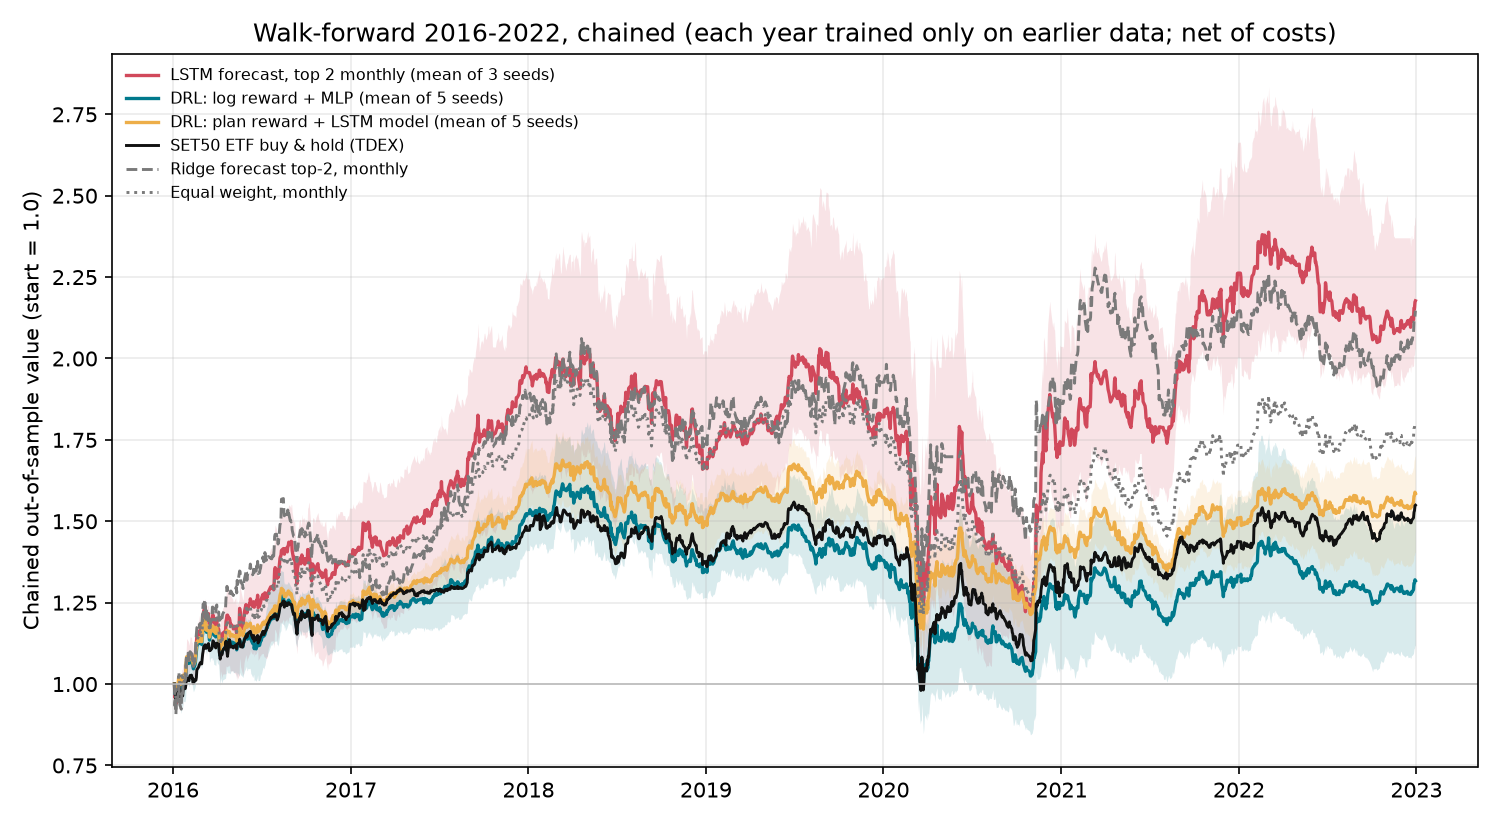
\includegraphics[width=\textwidth]{docs/figures/walk_forward_chained_equity_20261106.png}
\caption{Chained out-of-sample value over the seven validation years. Each year uses models trained only on earlier years. Bands show the range across seeds.}
\label{fig:walk-forward}
\end{figure}

Uncertainty was assessed on chained daily returns with a stationary block bootstrap~\cite{politis1994stationary},
the probabilistic Sharpe ratio~\cite{bailey2012sharpe}, and the deflated Sharpe ratio~\cite{bailey2014deflated},
counting the six designs screened earlier. The DRL LSTM agent had an annualized Sharpe ratio of 0.55
(95\% interval $-0.20$ to $1.32$) against 0.50 for the ETF. The paired difference was $+0.05$
(95\% interval $-0.29$ to $0.36$), and its deflated Sharpe ratio was 0.55, close to the value expected
from the best of six unskilled designs. The only difference whose interval excluded zero was that the
MLP agent was worse than equal weight (Sharpe difference $-0.24$, 95\% interval $-0.41$ to $-0.10$).

\section{Data-Source Ablation and Attribution}

With the reward, model, seeds, and folds fixed, the agent's inputs were varied (Table~\ref{tab:ablation}).

\begin{table}[H]
\centering
\small
\caption{Data-source ablation over the seven walk-forward years (three seeds per arm).}
\label{tab:ablation}
\begin{tabularx}{\textwidth}{@{}Yrrrr@{}}
\toprule
Inputs & Features & Annual return & vs ETF & Years ahead \\
\midrule
Technical only & 11 & 6.8\% & $-0.3\%$ & 3/7 \\
Technical + SET50 market context & 16 & 8.2\% & $+1.1\%$ & 4/7 \\
+ daily macro proxies & 24 & 7.1\% & $-0.1\%$ & 3/7 \\
\bottomrule
\end{tabularx}
\end{table}

\begin{figure}[H]
\centering
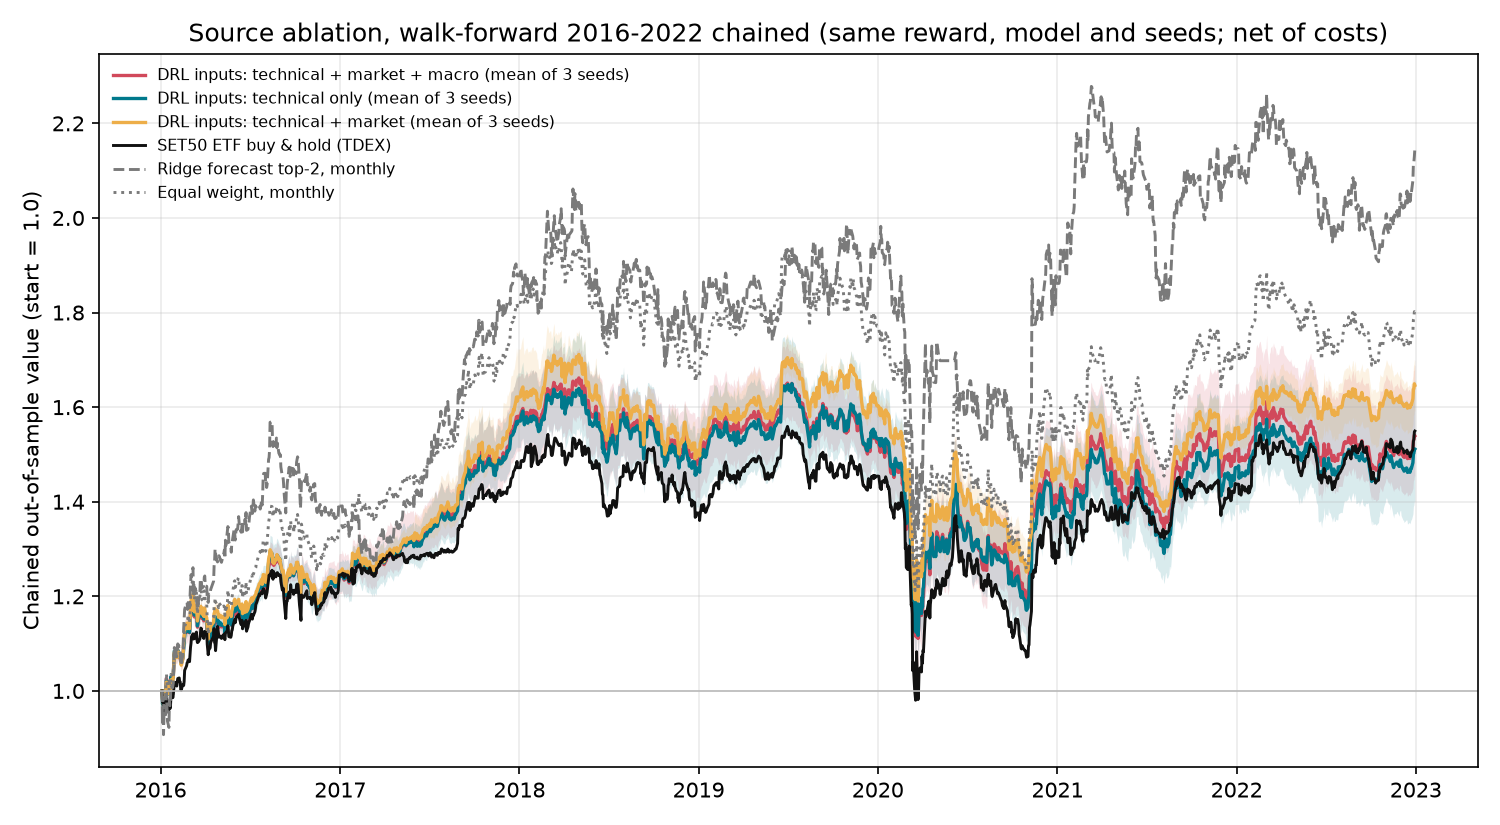
\includegraphics[width=\textwidth]{docs/figures/source_ablation_chained_equity_20261106.png}
\caption{Source ablation: chained out-of-sample value of the same DRL design with three input sets (three seeds each), compared with the ETF, equal weight, and the ridge forecast.}
\label{fig:ablation}
\end{figure}

Adding market context raised the Sharpe ratio by 0.10 relative to technical inputs only (95\% interval
$-0.002$ to $0.21$, one-sided $p=0.03$). That is borderline evidence, and it would not survive a
correction for the three comparisons. Daily macro proxies (USD/THB, Brent, gold, and the US 10-year
yield) added nothing.

Permutation attribution shuffled each source group in time and re-ran the trained agents. The macro
inputs moved the agent's weights by 2.9\%, the technical inputs by 5.5\%, and the market inputs by
1.9\%, but none changed annual return by more than 0.25 percentage points. In the main walk-forward
the LSTM agent's weights moved only 5.8\% (technical) and 2.5\% (market), so it behaved close to a
stable allocation. The MLP agent reacted strongly (27\% and 19\%) but lost more to trading costs (5.3\%
a year) than it gained from its inputs.

\section{Algorithm Comparison}

PPO was compared with A2C~\cite{mnih2016a3c} under the same reward, model, inputs, folds, and seeds
(Table~\ref{tab:algorithms}). PPO earned 0.9 percentage points more per year, beat the ETF in four of
seven years, and had the shallower drawdown. Most of its advantage came after the 2020 crash. The
Sharpe difference was not significant ($-0.11$ for A2C relative to PPO, 95\% interval $-0.26$ to
$0.04$). A2C trained about four times faster. The off-policy algorithms SAC~\cite{haarnoja2018sac},
TD3~\cite{fujimoto2018td3}, and DDPG~\cite{lillicrap2015ddpg} require about one hour per run and about
1~GB of replay memory with this model, so their comparison is prepared as an HPC array job rather
than run on the 8~GB development machine.

\begin{table}[H]
\centering
\small
\caption{On-policy algorithm comparison over the seven walk-forward years (three seeds each, same reward and model).}
\label{tab:algorithms}
\begin{tabularx}{\textwidth}{@{}Yrrrr@{}}
\toprule
Algorithm & Annual return & vs ETF & Years ahead & Max DD \\
\midrule
PPO & 8.2\% & $+1.1\%$ & 4/7 & $-11.1\%$ \\
A2C & 7.3\% & $+0.2\%$ & 3/7 & $-13.2\%$ \\
SET50 ETF buy-and-hold & 7.1\% & -- & -- & $-11.3\%$ \\
\bottomrule
\end{tabularx}
\end{table}

\section{Interpretation}

The long-term DRL design fixed the overtrading failure of the V2 objective. Over seven years it
roughly matched the SET50 market with the lowest drawdown of any strategy tested. However, it did not
outperform equal weighting of the same stocks or the supervised forecast-then-allocate baselines, and
no comparison among these strategies was statistically significant. The five starter stocks are
current large capitalization survivors chosen with hindsight, so even their equal-weight portfolio
outperformed the market index. Extending the evaluation to the point-in-time SET50/SET100 universe,
and adding fundamentals, news sentiment, investor flow, and official point-in-time macro data, are
required before any claim about Thai markets in general.
 immediately before
% \chapter{DISCUSSION}. It uses the report's own packages and column types (L, Y, booktabs, float).
% New references are in docs/report_drafts/references_additions_20261106.tex.
% Evidence tier: exploratory (Yahoo data, five starter stocks, validation years only). Numbers come
% from docs/long_term_reward_experiment_20261106.md, docs/walk_forward_reward_20261106.md and
% docs/source_ablation_20261106.md.

\chapter{LONG-TERM, MULTI-SOURCE EXTENSION}

This chapter reports experiments that align the implementation with the project title: a
\emph{long-term} objective, \emph{multi-source} inputs, and multi-year out-of-sample evaluation.
All results are exploratory. They use Yahoo Finance prices for the five starter stocks (ADVANC, AOT,
CPALL, KBANK, PTT) and the SET50 exchange-traded fund TDEX as the market series, because Yahoo now
returns only one row for the SET indices. Only validation years were read. The 2023--2024 test years
and the sealed post-2024 holdouts remain untouched for a single final evaluation after the protocol
is locked.

\section{Changes to the Environment and Objective}

The V2 environment charged turnover on the cash leg as well as on securities, so a 50\% purchase
from cash counted as 100\% turnover. It also reset portfolio weights to their targets after every
price move instead of letting them drift. Its reward was a one-day simple return minus a turnover
penalty of $0.05$ per unit of turnover, about fifty times the trading cost, and a penalty on the
\emph{level} of drawdown at every step. A new environment (\texttt{src/envs/long\_term\_env.py})
leaves the manifest-locked V2 files unchanged and adds opt-in options:

\begin{itemize}
  \item self-financing accounting with security-only turnover, multiplicative costs, and drifting weights;
  \item a log-wealth reward $\log(1+R_t)$, whose sum over an episode equals log terminal wealth;
  \item the plan reward $\alpha\log(1+R_t)+\beta D_t-\gamma\,\Delta\mathrm{DD}_t-\lambda\,\mathrm{TO}_t$, where $D_t$ is the differential Sharpe ratio of Moody and Saffell~\cite{moody2001drl} and only \emph{increases} in drawdown are penalized;
  \item a rebalancing interval, random two-year training episodes, and softmax portfolio weights with an explicit cash share.
\end{itemize}

With default options the new environment reproduced the V2 environment exactly. A randomized test
compares observations, rewards, and diagnostic values on random configurations. Trading costs were
set to 0.15\% commission plus 0.05\% slippage per side. That covers the published explicit cost of
about 0.176\% per side: a 0.157\% internet commission, SET, TSD, and SEC fees, and 7\% VAT.

\section{Reward and Rebalancing Designs (2020--2022)}

Six designs were trained with PPO for 100{,}000 timesteps and three seeds on 2012--2019. They were
evaluated on 2020--2022, which includes the COVID-19 crash, under self-financing accounting
(Table~\ref{tab:reward-designs}).

\begin{table}[H]
\centering
\small
\caption{Reward and rebalancing designs, validation 2020--2022 (mean $\pm$ s.d. over three seeds). Max DD is maximum drawdown, turnover is per session, and costs are commission plus slippage summed over the period as a share of portfolio value.}
\label{tab:reward-designs}
\begin{tabularx}{\textwidth}{@{}Yrrrr@{}}
\toprule
Design & Return & Max DD & Turnover & Costs \\
\midrule
V2 objective & $-48.8\% \pm 7.6$ & $-50.7\%$ & 0.519 & 75.3\% \\
Daily simple return, fixed accounting & $-41.9\% \pm 6.9$ & $-44.6\%$ & 0.386 & 56.0\% \\
Log return, weekly & $-2.8\% \pm 5.8$ & $-28.6\%$ & 0.110 & 16.0\% \\
Plan reward, weekly & $-8.8\% \pm 17.2$ & $-28.0\%$ & 0.081 & 11.7\% \\
Log return, monthly & $-5.2\% \pm 5.3$ & $-30.4\%$ & 0.031 & 4.5\% \\
Plan reward, weekly, LSTM model & $+1.9\% \pm 1.1$ & $-26.0\%$ & 0.011 & 1.6\% \\
\midrule
SET50 ETF buy-and-hold & $+9.0\%$ & $-32.6\%$ & -- & 0.2\% \\
Ridge forecast, top two, monthly & $+4.9\%$ & $-33.2\%$ & 0.050 & 7.3\% \\
Equal weight, monthly & $+2.7\%$ & $-31.6\%$ & 0.003 & 0.5\% \\
\bottomrule
\end{tabularx}
\end{table}

The V2 objective lost money mainly through overtrading: its policy turned over the portfolio about
377 times in three years. Correcting the accounting alone did not help, because a daily-decision agent
still churned. Long-horizon rewards with weekly or monthly decisions cut costs by 79--94\% and
reduced the loss from about 49\% to about 3\%. A shared per-asset LSTM encoder of each stock's
\emph{past} window (\texttt{asset\_lstm}) gave the only design that was positive on every seed.

\section{Seven-Year Walk-Forward Evaluation}

The two carried-forward designs were re-evaluated with seven expanding folds. Each fold trained on
2012 through December of year $Y-1$ and validated on year $Y$ ($Y=2016,\dots,2022$), with five seeds per
design. Two supervised forecast-then-allocate baselines were fitted on the same training dates: a ridge
regression and a bidirectional LSTM over each stock's past window. Each predicted 21-session returns
and bought its top two forecasts monthly. Table~\ref{tab:walk-forward} summarizes the folds.

\begin{table}[H]
\centering
\small
\caption{Walk-forward validation 2016--2022: mean over seven annual folds (DRL: five seeds per fold).}
\label{tab:walk-forward}
\begin{tabularx}{\textwidth}{@{}Yrrrr@{}}
\toprule
Strategy & Annual return & vs ETF & Years ahead & Max DD \\
\midrule
LSTM forecast, top two & 13.8\% & $+6.7\%$ & 5/7 & $-17.0\%$ \\
Ridge forecast, top two & 12.8\% & $+5.6\%$ & 5/7 & $-16.8\%$ \\
Equal weight, monthly & 10.1\% & $+3.0\%$ & 4/7 & $-13.9\%$ \\
DRL, plan reward + LSTM model & 7.7\% & $+0.5\%$ & 3/7 & $-11.1\%$ \\
SET50 ETF buy-and-hold & 7.1\% & -- & -- & $-11.3\%$ \\
DRL, log reward + MLP & 5.0\% & $-2.2\%$ & 2/7 & $-14.2\%$ \\
\bottomrule
\end{tabularx}
\end{table}

\begin{figure}[H]
\centering
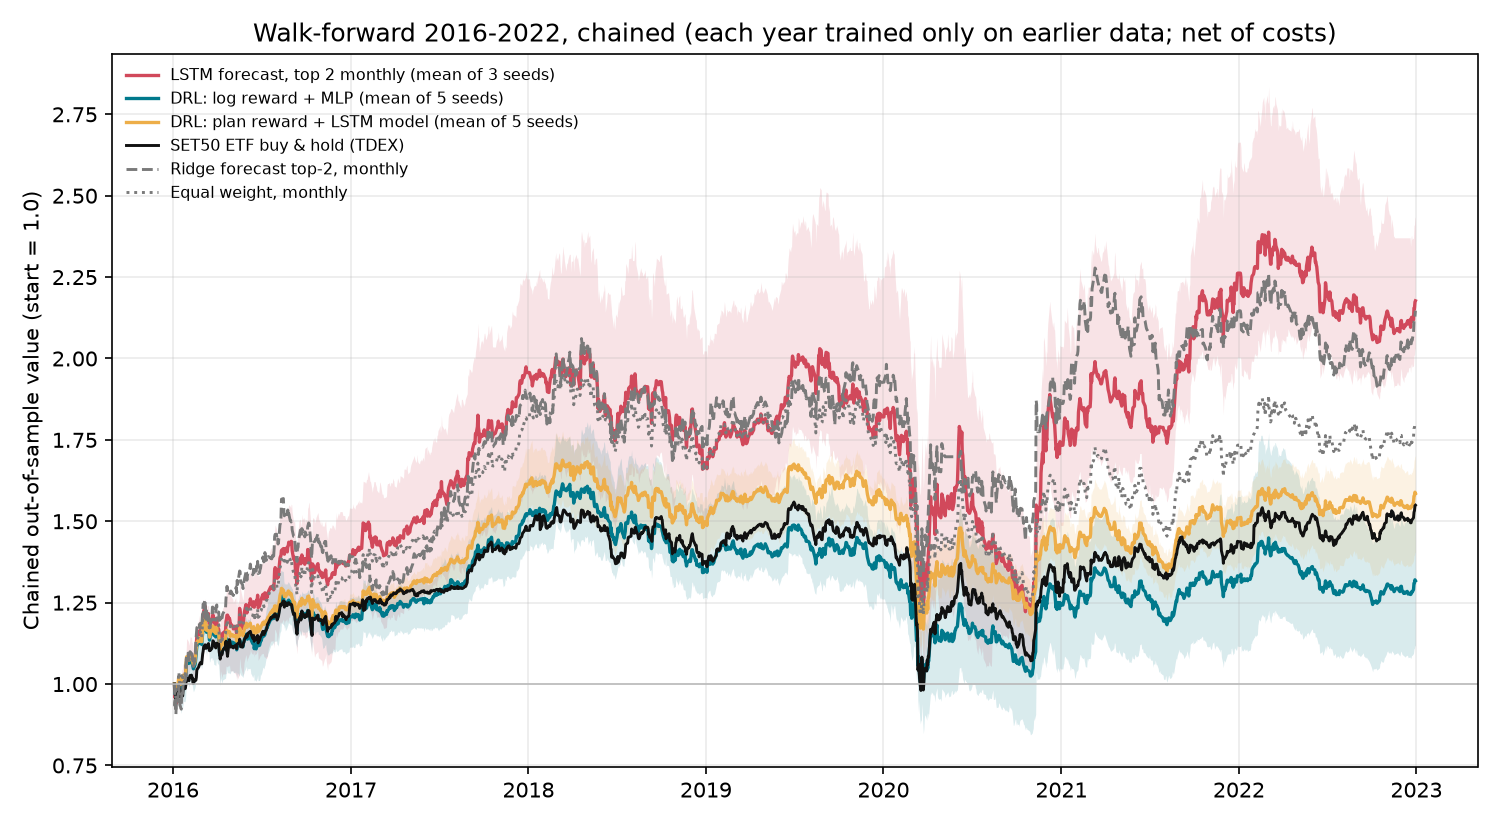
\includegraphics[width=\textwidth]{docs/figures/walk_forward_chained_equity_20261106.png}
\caption{Chained out-of-sample value over the seven validation years. Each year uses models trained only on earlier years. Bands show the range across seeds.}
\label{fig:walk-forward}
\end{figure}

Uncertainty was assessed on chained daily returns with a stationary block bootstrap~\cite{politis1994stationary},
the probabilistic Sharpe ratio~\cite{bailey2012sharpe}, and the deflated Sharpe ratio~\cite{bailey2014deflated},
counting the six designs screened earlier. The DRL LSTM agent had an annualized Sharpe ratio of 0.55
(95\% interval $-0.20$ to $1.32$) against 0.50 for the ETF. The paired difference was $+0.05$
(95\% interval $-0.29$ to $0.36$), and its deflated Sharpe ratio was 0.55, close to the value expected
from the best of six unskilled designs. The only difference whose interval excluded zero was that the
MLP agent was worse than equal weight (Sharpe difference $-0.24$, 95\% interval $-0.41$ to $-0.10$).

\section{Data-Source Ablation and Attribution}

With the reward, model, seeds, and folds fixed, the agent's inputs were varied (Table~\ref{tab:ablation}).

\begin{table}[H]
\centering
\small
\caption{Data-source ablation over the seven walk-forward years (three seeds per arm).}
\label{tab:ablation}
\begin{tabularx}{\textwidth}{@{}Yrrrr@{}}
\toprule
Inputs & Features & Annual return & vs ETF & Years ahead \\
\midrule
Technical only & 11 & 6.8\% & $-0.3\%$ & 3/7 \\
Technical + SET50 market context & 16 & 8.2\% & $+1.1\%$ & 4/7 \\
+ daily macro proxies & 24 & 7.1\% & $-0.1\%$ & 3/7 \\
\bottomrule
\end{tabularx}
\end{table}

\begin{figure}[H]
\centering
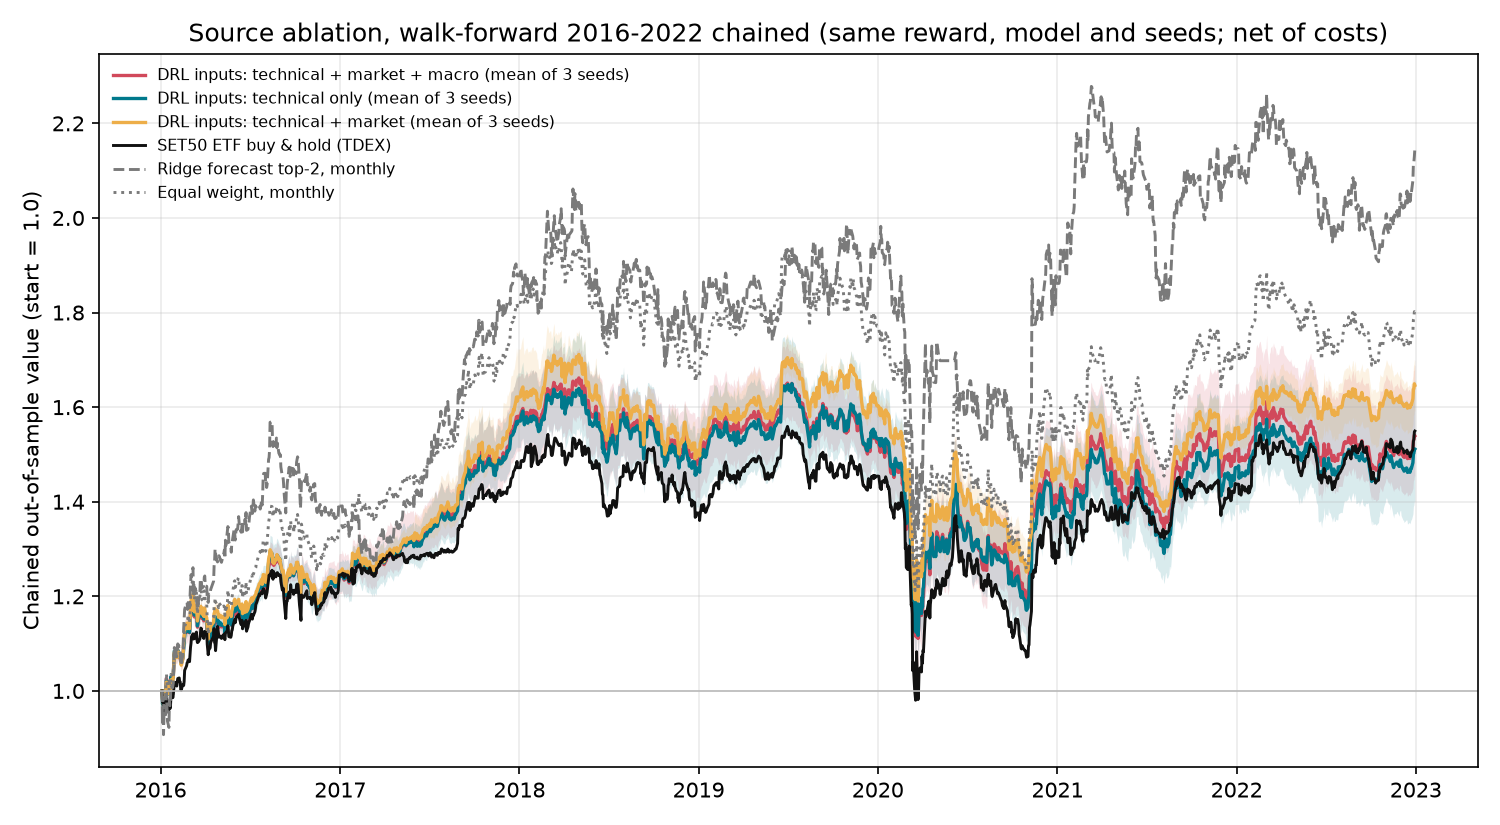
\includegraphics[width=\textwidth]{docs/figures/source_ablation_chained_equity_20261106.png}
\caption{Source ablation: chained out-of-sample value of the same DRL design with three input sets (three seeds each), compared with the ETF, equal weight, and the ridge forecast.}
\label{fig:ablation}
\end{figure}

Adding market context raised the Sharpe ratio by 0.10 relative to technical inputs only (95\% interval
$-0.002$ to $0.21$, one-sided $p=0.03$). That is borderline evidence, and it would not survive a
correction for the three comparisons. Daily macro proxies (USD/THB, Brent, gold, and the US 10-year
yield) added nothing.

Permutation attribution shuffled each source group in time and re-ran the trained agents. The macro
inputs moved the agent's weights by 2.9\%, the technical inputs by 5.5\%, and the market inputs by
1.9\%, but none changed annual return by more than 0.25 percentage points. In the main walk-forward
the LSTM agent's weights moved only 5.8\% (technical) and 2.5\% (market), so it behaved close to a
stable allocation. The MLP agent reacted strongly (27\% and 19\%) but lost more to trading costs (5.3\%
a year) than it gained from its inputs.

\section{Algorithm Comparison}

PPO was compared with A2C~\cite{mnih2016a3c} under the same reward, model, inputs, folds, and seeds
(Table~\ref{tab:algorithms}). PPO earned 0.9 percentage points more per year, beat the ETF in four of
seven years, and had the shallower drawdown. Most of its advantage came after the 2020 crash. The
Sharpe difference was not significant ($-0.11$ for A2C relative to PPO, 95\% interval $-0.26$ to
$0.04$). A2C trained about four times faster. The off-policy algorithms SAC~\cite{haarnoja2018sac},
TD3~\cite{fujimoto2018td3}, and DDPG~\cite{lillicrap2015ddpg} require about one hour per run and about
1~GB of replay memory with this model, so their comparison is prepared as an HPC array job rather
than run on the 8~GB development machine.

\begin{table}[H]
\centering
\small
\caption{On-policy algorithm comparison over the seven walk-forward years (three seeds each, same reward and model).}
\label{tab:algorithms}
\begin{tabularx}{\textwidth}{@{}Yrrrr@{}}
\toprule
Algorithm & Annual return & vs ETF & Years ahead & Max DD \\
\midrule
PPO & 8.2\% & $+1.1\%$ & 4/7 & $-11.1\%$ \\
A2C & 7.3\% & $+0.2\%$ & 3/7 & $-13.2\%$ \\
SET50 ETF buy-and-hold & 7.1\% & -- & -- & $-11.3\%$ \\
\bottomrule
\end{tabularx}
\end{table}

\section{Interpretation}

The long-term DRL design fixed the overtrading failure of the V2 objective. Over seven years it
roughly matched the SET50 market with the lowest drawdown of any strategy tested. However, it did not
outperform equal weighting of the same stocks or the supervised forecast-then-allocate baselines, and
no comparison among these strategies was statistically significant. The five starter stocks are
current large capitalization survivors chosen with hindsight, so even their equal-weight portfolio
outperformed the market index. Extending the evaluation to the point-in-time SET50/SET100 universe,
and adding fundamentals, news sentiment, investor flow, and official point-in-time macro data, are
required before any claim about Thai markets in general.
